\subsection{Hidden Markov Models}

HMMs describe time series with state-switching behaviour. An HMM models an observed sequence of length $T$, $\bfY = \{Y_t\}_{t=1}^T$, together with an unobserved (or  ``hidden") sequence $\bfX = \{X_t\}_{t=1}^T$. The hidden sequence $\bfX$ is Markov chain, and each observation $Y_t$ is a random variable whose distribution depends only on its corresponding hidden state $X_t$. While the sample space of $\bfX$ is general, we assume $X_t \in \{1,\ldots,N\}$ for some finite $N$. The unconditional distribution of $X_1$ is denoted by the row-vector $\delta \in \bbR^N$, where $\delta^{(i)} = \bbP(X_t = i)$. Further, the distribution of $X_t$ for $t > 1$ conditioned on $X_{t-1}$ is denoted by an $N$-by-$N$ transition probability matrix $\Gamma_t$, where $\Gamma_t^{(i,j)} = \bbP(X_t = j \mid X_{t-1} = i)$. Our methods apply to transition probability matrices which depend upon time, but for ease of presentation we assume that $\Gamma_t$ does not change over time (i.e. $\Gamma_t = \Gamma$ for all $t$) unless stated otherwise. 

We assume that the distribution of an observation $Y_t$ conditioned on the corresponding hidden state $X_t$ does not depend upon any other observation or hidden state.
%Some variants of HMMs allow $Y_t$ to depend upon both $Y_{t-1}$ and $X_t$. Our methodology can be straightforwardly applied to such HMMs, but for clarity of presentation we assume that $Y_t$ depends only on $X_t$. 
If $X_t=i$, then we denote the conditional density or probability mass function of $Y_t$ as $f^{(i)}(\cdot ; \theta^{(i)})$ or simply $f^{(i)}(\cdot)$, where $\theta^{(i)}$ is a state-dependent parameter describing the emission distribution. Figure \ref{fig:HMM} shows an HMM as a graphical model.

\begin{figure}[h]
    \centering
    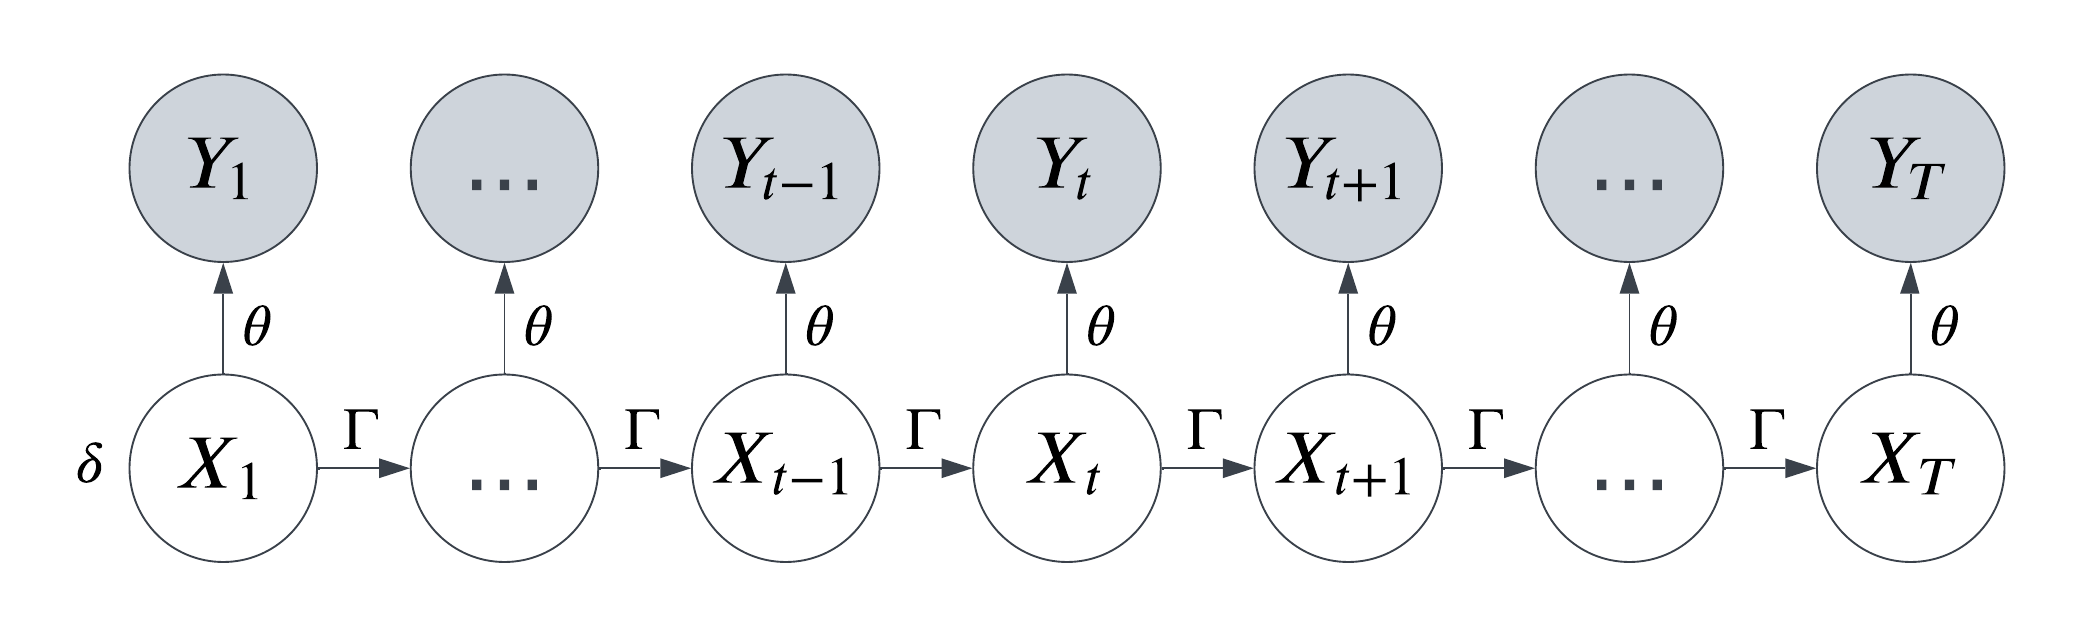
\includegraphics[width=5in]{../plt/HMM.png}
    \caption{Graphical representation of an HMM. $X_t$ corresponds to an unobserved latent state at time $t$ which follows a Markov chain, and $Y_t$ corresponds to an observation at time $t$ that is independent of all other random variables when conditioned on $X_t$.}
    \label{fig:HMM}
\end{figure}

It is convenient to reparameterize the transition probability matrix $\Gamma \in \bbR^{N \times N}$ and initial distribution $\delta \in \bbR^N$ in terms of an auxiliary variable $\eta$ to ensure that all entries are positive and all rows sum to one. One option is to follow the parameterization of \citet{Barajas:2017}:
%
\begin{equation}
    \Gamma^{(i,j)}(\eta) = \frac{\exp(\eta^{(i,j)})}{\sum_{k=1}^N \exp(\eta^{(i,k)})}, \qquad \delta^{(i)}(\eta) = \frac{\exp(\eta^{(i)})}{\sum_{k=1}^N \exp(\eta^{(k)})}
    \label{eqn:reparam}
\end{equation}
%
where $i,j = 1,\ldots,N$ and $\eta^{(i,i)}$ and $\eta^{(1)}$ are set to zero for identifiability. This formulation simplifies likelihood maximization by removing constraints in the optimization problem. One may also incorporate covariates into $\Gamma$ by setting $\eta_t^{(i,j)}(\beta) = \left(\beta^{(i,j)}\right)^T z_t$, where $z_t$ is a column vector of known covariates and $\beta^{(i,j)}$ is a column vector of unknown regression coefficients. While $\Gamma$ and $\delta$ are functions of $\eta$, we abuse notation in future sections and treat $\Gamma$ and $\delta$ as variables since the mapping is a bijection.

The joint likelihood of some fixed observed data $\bfy$ and given latent states $\bfx$ is
%
\begin{equation}
    p(\bfx,\bfy;\theta,\eta) = \delta^{(x_1)} f^{(x_1)}(y_1; \theta^{(x_1)}) \prod_{t=2}^T \Gamma^{(x_{t-1},x_t)} f^{(x_t)}(y_t; \theta^{(x_t)}).
    \label{eqn:like}
\end{equation}
%
Alternatively, the marginal likelihood of the observed data $\bfy$ alone is 
%
\begin{equation}
    p(\bfy;\theta,\eta) = \delta P(y_1;\theta) \prod_{t=2}^T \Gamma P(y_t;\theta) \mathbf{1}_N.
    \label{eqn:like_marginal}
\end{equation}
%
where $\mathbf{1}_N$ is an $N$-dimensional column vector of ones and $P(y_t;\theta)$ is an $N \times N$ diagonal matrix with the $(i,i)^{th}$ entry $f^{(i)}(y_t; \theta^{(i)})$.

\subsection{Hierarchical Hidden Markov Models}

The transition probability matrix $\Gamma$ can be parameterized to enforce a hierarchical structure \citep{Barajas:2017}. In particular, define a coarse-scale initial distribution $\delta_c \in \bbR^{N_c}$, a coarse-scale probability transition matrix ($\boldsymbol{\Gamma}_c \in \bbR^{{N_c} \times {N_c}}$), ${N_c}$ fine-scale initial distributions $\{\delta_f^{(i)}\}_{i=1}^{N_c}$, each in $\bbR^{N_f^{(i)}}$, and ${N_c}$ fine-scale transition probability matrices $\{\boldsymbol{\Gamma}_f^{(i)}\}_{i=1}^{N_c}$, each in $\bbR^{N_f^{(i)} \times N_f^{(i)}}$. Each initial distribution and probability matrix is parameterized similarly to Equation (\ref{eqn:reparam}). Further, define the matrix $\boldsymbol{\Pi}_f^{(i)}$ as an $N_f^{(i)} \times N_f^{(i)}$ matrix with identical row entries, $\delta_f^{(i)}$, the initial distribution over fine-scale states for the $i^{th}$ coarse-scale state. Then, the global probability transition matrix $\boldsymbol{\Gamma}$ is the following: %\textcolor{red}{I stole this from Vianey}:

\begin{equation} 
\boldsymbol{\Gamma} = 
\begin{pmatrix}
\Gamma_c^{(1,1)}\boldsymbol{\Gamma}_f^{(1)}     & \Gamma_c^{(1,2)} \boldsymbol{\Pi}_f^{(2)}     & \cdots & \Gamma_c^{(1,N_c)}\boldsymbol{\Pi}_f^{(N_c)}  \cr
\Gamma_c^{(2,1)}\boldsymbol{\Pi}_f^{(1)} & \Gamma_c^{(2,2)} \boldsymbol{\Gamma}_f^{(2)}  & \cdots & \Gamma_c^{(2,N_c)}\boldsymbol{\Pi}_f^{(N_c)} \cr
\vdots & \vdots & \ddots & \vdots \cr 
\Gamma_c^{(N_c,1)}\boldsymbol{\Pi}_f^{(1)} & \Gamma_c^{(N_c,2)}\boldsymbol{\Pi}_f^{(2)}      & \cdots & \Gamma_c^{(N_c,N_c)} \boldsymbol{\Gamma}_f^{(N_c)} 
\end{pmatrix}.
\label{exptpm2}
\end{equation}

A model with a transition probability matrix in the form of (\ref{exptpm2}) is known as a hierarchical hidden Markov model, or HHMM. The total number of hidden states for an HHMM is $N = \sum_{i=1}^{N_c} N_f^{(i)}$ and the transition probability matrix $\Gamma$ of a hierarchical HMM is simply a more restricted version of the probability transition matrix from a traditional HMM.

\subsection{State Decoding}

One appealing feature of an HMM is that it is possible to determine the probability distribution of the hidden state at time $t$, $X_t$, conditional of the set of observations $Y_t$. To this end, we define the probability density of the observations between times $s$ and $t$ as $p(y_{s:t};\theta,\eta)$. We also define \textit{forward probabilities} $\alpha^{(i)}_t = p(y_{1:t},X_t = i;\theta,\eta)$ (for $i = 1,\ldots,N$ and $t = 1,\ldots,T$) and \textit{backward probabilities} $\beta^{(i)}_t = p(y_{(t+1):T}|X_t = i;\theta,\eta)$ (for $i = 1,\ldots,N$ and $t = 1,\ldots,T-1$). By convention, $\beta^{(i)}_T = 1$ for $i = 1,\ldots,N$. 
Both $\alpha_t$ and $\beta_t$ can be defined recursively:
%
\begin{align}
    \alpha_1^{(i)}(\theta,\eta) &= \delta^{(i)} f^{(i)}(y_1;\theta), & \alpha_t^{(i)}(\theta,\eta) &= \sum_{j=1}^N \alpha_{t-1}^{(j)} \Gamma^{(j,i)}(\eta) f^{(i)}(y_t;\theta^{(i)}), \quad t = 2,\ldots,T. \label{eqn:alpha} \\
    %
    \beta_T^{(i)}(\theta,\eta) &= 1, & \beta_t^{(i)}(\theta,\eta) &= \sum_{j=1}^N \Gamma^{(i,j)} f^{(j)}(y_{t+1};\theta) \beta^{(j)}_{t+1}, \quad t = 1,\ldots,T-1. \label{eqn:beta}
\end{align}

We denote the probability that $X_t = i$ given all observations $\bfy$ and parameters $\{\theta,\eta\}$ as $\gamma_t^{(i)}(\theta,\eta)$ for $t = 1,\ldots,T$ and $i = 1,\ldots,N$. Further, we denote the probability that $X_{t-1} = i$ and $X_t = j$ given all observations $\bfy$ and parameters $\{\theta,\eta\}$ as $\xi_t^{(i,j)}(\theta,\eta)$ for $t = 2,\ldots,T$ and $i,j = 1,\ldots,N$. Namely,
%
\begin{gather*}
    \gamma_t^{(i)}(\theta,\eta) = \bbP(X_t = i \mid \bfy ~;~ \theta,\eta), \\ \xi_t^{(i,j)}(\theta,\eta) = \bbP(X_{t-1} = i, X_t = j \mid \bfy ~;~ \theta,\eta). \nonumber
\end{gather*}
%
Both $\gamma_t$ and $\xi_t$ can be calculated from $\alpha_{t-1}$, $\alpha_t$, and $\beta_t$:
%
\begin{gather}
    \gamma_{t}^{(i)}\big(\theta,\eta\big) = \frac{\alpha_{t}^{(i)} ~ \beta_{t}^{(i)}}{\sum_{i'} \alpha_{t}^{(i')} ~ \beta_{t}^{(i')}}, \label{eqn:gamma} \\
    %
    \xi_{t}^{(i,j)}\big(\theta, \eta) = \frac{\alpha_{t-1}^{(i)} ~ \Gamma^{(i,j)} ~ f^{(j)}(y_{t} ~ ; ~\theta) ~ \beta_{t}^{(j)}}{\sum_{i',j'} ~ \alpha_{t-1}^{(i')} ~ \Gamma^{(i',j')}(\eta) ~ f^{(j')}(y_{t} ~ ; ~\theta) ~ \beta_{t}^{(j')}} \label{eqn:xi},
\end{gather}

\subsection{The Baum-Welch Algorithm}

The Baum-Welch algorithm is an optimization technique is used to estimate the parameters of the HMM. It is simply the specific instance of the EM algorithm when applied to HMMs. Suppose a sequence of observations $\bfy$ is observed as output of an HMM with unknown latent states $\bfX$ and unknown parameters $\{\theta,\eta\}$. Define the function $Q(\theta,\eta \mid \theta[k],\eta[k])$ as the expected value of the joint log-likelihood $\log p(\bfy,\bfX; \theta,\eta)$ when $\bfX$ is a random variable with density $p(\bfX | \bfy;\theta[k],\eta[k])$. The Baum-Welch algorithm updates the parameter estimates at step $k+1$ by maximizing $Q(\theta,\eta \mid \theta[k],\eta[k])$ with respect to the parameters $\{\theta,\eta\}$:
%
\begin{gather}
    \left\{\theta[k+1],\eta[k+1]\right\} = \argmax_{\theta,\eta} Q(\theta,\eta \mid \theta[k],\eta[k]), \\
    %
    Q(\theta,\eta \mid \theta[k],\eta[k]) \equiv \bbE_{p(\bfX \mid \bfy;\theta[k],\eta[k])}\left[\log p(\bfy,\bfX;\theta,\eta) \right]
    \label{eqn:BW_update}
\end{gather}
%
We can combine Equation (\ref{eqn:BW_update}) with Equation (\ref{eqn:like}) to separate the expected value into three convenient terms:
\begin{align*}
    \bbE_{p(\bfX \mid \bfy;\theta[k],\eta[k])}\left[\log p(\bfy,\bfX;\theta,\eta) \right] &= \bbE_{p(\bfX \mid \bfy;\theta[k],\eta[k])} \left[\log \delta^{(X_1)} + \sum_{t=1}^T \log f^{(X_t)}(y_t;\theta^{(X_t)}) + \sum_{t=2}^{T} \log \Gamma^{(X_{t-1},X_{t})} \right] \\
    %
    &= \bbE_{p(\bfX \mid \bfy;\theta[k],\eta[k])} \Big[\log \delta_{X_1}\Big] \\ & \qquad + \sum_{t = 1}^T \bbE_{p(\bfX \mid \bfy;\theta[k],\eta[k])} \left[ \log f^{(X_t)}(y_t;\theta^{(X_t)})\right] \\ & \qquad + \sum_{t=2}^{T} \bbE_{p(\bfX \mid \bfy;\theta[k],\eta[k])} \left[ \log \Gamma^{(X_{t-1},X_{t})} \right] \\
    %
    &= \sum_{i=1}^N \gamma^{(i)}_1(\theta[k],\eta[k]) \log \delta^{(i)} \\ & \qquad + \sum_{t = 1}^T \sum_{i=1}^N \gamma^{(i)}_t(\theta[k],\eta[k]) \log f^{(i)}(y_t;\theta^{(i)}) \\
    & \qquad + \sum_{t=2}^{T} \sum_{i=1}^N \sum_{j=1}^N \xi_t^{(i,j)}(\theta[k],\eta[k]) \log \Gamma^{(i,j)}.
\end{align*}

Each of the three terms on the RHS of the equation above only depend upon $\delta$, $\theta$, and $\Gamma$, respectively. As a result, the maximization problem can be divided into three separate sub-problems:
%
\begin{gather}
    \delta[k+1] = \argmax_{\delta} \sum_{i=1}^N \gamma^{(i)}_1(\theta[k],\eta[k]) \log \delta^{(i)} \label{eqn:EM_update_delta} \\
    %
    \theta[k+1] = \argmax_{\theta} \sum_{t = 1}^T \sum_{i=1}^N \gamma^{(i)}_t(\theta[k],\eta[k]) \log f^{(i)}(y_t;\theta^{(i)}) \label{eqn:EM_update_theta} \\
    %
    \Gamma[k+1] = \argmax_{\Gamma} \sum_{t=2}^{T} \sum_{i=1}^N \sum_{j=1}^N \xi_t^{(i,j)}(\theta[k],\eta[k]) \log \Gamma^{(i,j)} \label{eqn:EM_update_Gamma}
\end{gather}
%
In many simple scenarios the maximization problems above have closed-form solutions. For example, if $\Gamma$ does not depend upon any covariates and $f^{(i)}(y_t;\theta^{(i)})$ is a normal or Poisson probability density function with respect to $y_t$, then the solutions of Equations (\ref{eqn:EM_update_delta}--\ref{eqn:EM_update_Gamma}) are given in Section 4.2 of \citet{Zucchini:2016}. However, in many other situations (e.g. if $\Gamma$ or $f^{(i)}$ depend upon covariates), the maximization problem above is not straightforward and requires numerical maximization techniques. Whether or not Equations (\ref{eqn:EM_update_delta}--\ref{eqn:EM_update_Gamma}) have closed-form solutions, even defining the optimization problem (the E-step) has a time cost of $\calO(T)$, which can be expensive for large $T$. 

\subsection{Direct likelihood maximization}

An alternative way to perform inference over HMMs is to directly maximize the marginal likelihood from Equation (\ref{eqn:like_marginal}) using gradient-based optimization techniques. One standard method is gradient descent, which updates $\theta$ or $\eta$ at step $m$ using the following update rule with step sizes $\lambda^\eta$ and $\lambda^\theta$:
%
\begin{gather}
    \eta[m+1] = \eta[m] + \lambda^{\eta} \nabla_\eta \log p(\bfy;\theta[m],\eta[m]) \\
    %
    \theta[m+1] = \theta[m] + \lambda^{\theta} \nabla_\theta \log p(\bfy;\theta[m],\eta[m]).
    \label{eqn:grad_update}
\end{gather}
%
Using the Fisher identity of the gradient for incomplete data models \citep{Fisher:1925}, the gradient of Equation (\ref{eqn:like_marginal}) can be written as
%
\begin{equation}
    \nabla_{\theta,\eta} \log p(\bfy;\theta,\eta) = \bbE_{p(\bfX \mid \bfy;\theta,\eta)}\left[ \nabla_{\theta,\eta} \log p(\bfy,\bfX;\theta,\eta) \right].
    \label{eqn:fisher_id}
\end{equation}
%
Similarly to the EM algorithm, we can split the gradient of the log-likelihood into separate terms that each depend on only $\theta$ or $\eta$:
%
\begin{gather}
    \nabla_{\theta} \log p(\bfy;\theta,\eta) = \sum_{t=1}^T \sum_{i=1}^N \gamma_t^{(i)}(\theta,\eta) \nabla_{\theta} \log f^{(i)}(y_t;\theta^{(i)}) \label{eqn:theta_update_gd} \\
    %
    \nabla_{\eta} \log p(\bfy;\theta,\eta) = \sum_{i=1}^N \gamma_1^{(i)}(\theta,\eta) \nabla_{\eta} \log \delta^{(i)} + \sum_{t=2}^{T} \sum_{i=1}^N \sum_{j=1}^N \xi_t^{(i,j)}(\theta,\eta) \nabla_{\eta} \log \Gamma^{(i,j)}, \label{eqn:eta_update_gd}
\end{gather}
%
There is a clear connection between the Baum-Welch update from Equation (\ref{eqn:BW_update}) and the gradient given by Equation (\ref{eqn:fisher_id}). In particular, one recovers gradient descent by performing one gradient step within the M-step of the Baum-Welch algorithm rather than solving the entire maximization problem. This connection leads to a natural question: if taking one gradient step within the M- step is equivalent to gradient descent, and solving the M- step entirely results in the Baum-Welch algorithm, then are there other ways to perform the M-step in the EM algorithm with desirable properties? To answer this question, we first review some stochastic optimization techniques.

\subsection{Stochastic Optimization}

Stochastic optimization techniques are useful to solve optimization problems of the following form:
%
\begin{equation*}
    \min P(z), \qquad P(z) = \frac{1}{T}\sum_{t = 1}^T P_t(z).
\end{equation*}
%
Standard gradient descent updates $z$ at step $m$ using the following update rule with step size $\lambda$:
%
\begin{equation*}
    z[m+1] = z[m] - \lambda \nabla P(z[m]) =  z[m] - \frac{\lambda}{T} \sum_{t=1}^T \nabla P_t(z[m]).
\end{equation*}
%
However, this update requires evaluating a gradient for all $t = 1,\ldots,T$, which can be prohibitive if $T$ is large. Alternatively, \citet{Robbins:1951} introduce stochastic gradient descent (or SGD), which updates $z$ using an unbiased estimate of the full gradient:
%
\begin{equation*}
    z[m+1] = z[m] - \lambda \nabla P_{t_m}(z[m])
\end{equation*}
%
for some $t_m \in \{1,\ldots,T\}$ selected uniformly at random at step $m$. Stochastic gradient descent reduces the amount of time between updates by using an unbiased estimate of the gradient to update $z[m]$. However, the gradient estimates themselves can have high variance, so stochastic gradient descent requires that the step-size $\lambda$ decays over time to ensure convergence. In addition, SGD has slower convergence rates compared to full gradient descent \citep{Schmidt:2017}.

Recent variance-reduced stochastic optimization techniques including (but not limited to) SAG \citep{Schmidt:2017}, SVRG \citep{Johnson:2013}, and SAGA \citep{Defazio:2014} enjoy the speed of stochastic gradient descent as well as the convergence rates of full gradient descent. These algorithms involve storing a table of gradient \textit{estimates} $\widehat \nabla P_t$ that are updated and stored at various stages in the optimization algorithm. The table average then approximates the full gradient $\nabla P(z[m])$. The gradient estimate can be used to reduce the variance of future gradient estimates. In particular, SAG uses the update rule:
%
\begin{equation}
    z[m+1] \gets z[m] - \lambda \left[\frac{\nabla P_{t_m}(z[m]) - \widehat \nabla P_{t_m}}{T} + \frac{1}{T} \sum_{t=1}^T \widehat \nabla P_{t} \right], \label{eqn:SAG_update}
\end{equation}
%
which is simply the table average with entry $t_m$ updated at step $m$. This update rule is intuitive, but it represents a biased estimate of the gradient $\nabla P(z)$. This can slow down convergence and makes theoretical analysis of SAG difficult. SVRG and SAGA, on the other hand, utilize an unbiased estimate of the gradient to update $z$:
%
\begin{equation}
    z[m+1] \gets z[m] - \lambda \left[\nabla P_{t_m}(z[m]) - \widehat \nabla P_{t_m} + \frac{1}{T} \sum_{t=1}^T \widehat \nabla P_{t} \right].
    \label{eqn:SAGA_update}
\end{equation}
%
Taking the expected value of the gradient estimate from (\ref{eqn:SAGA_update}) shows that it is unbiased:
%
\begin{align*}
    \bbE\left[\nabla P_{t_m}(z[m]) - \widehat \nabla P_{t_m} + \frac{1}{T} \sum_{t=1}^T \widehat \nabla P_{t} \right] &= \frac{1}{T} \sum_{t=1}^T \nabla P_{t}(z[m]) - \frac{1}{T} \sum_{t=1}^T \widehat \nabla P_{t} + \frac{1}{T} \sum_{t=1}^T \widehat \nabla P_{t} \\
    %
    &= \frac{1}{T} \sum_{t=1}^T \nabla P_{t_m}(z[m]) = \nabla P(z[m]).
\end{align*}
%
After updating the parameters at step $m$, SAG and SAGA simply update the table at position $t_m$: 
%
\begin{equation}
    \widehat \nabla P_{t_m} \leftarrow \nabla P_{t_m}(z[m]).
\end{equation}
%
%After updating the table at position $t_m$ with the SAG/SAGA update rule, the table average $\frac{1}{T} \sum_{t=1}^T \widehat \nabla P_{t}$ must be updated using the previous estimate of $\widehat \nabla P_{t}$. 
Both SAG and SAGA can be memory intensive because the gradient at every index must be stored. On the other hand, SVRG updates the \textit{entire} table average once every $M$ iterations and recalculates the table entries $\widehat \nabla P_{t_m}$ as needed. As such, SVRG saves memory since it does not store gradient estimates at each index. However, SVRG recalculates table entries at every parameter update, so it can be more computationally expensive than SAGA and SAG. 

In summary, SVRG is less memory intensive, but more computationally expensive compared to SAGA. This trade-off should be considered by practitioners when deciding between the two algorithms. In addition, SVRG's table average is updated less often compared to SAGA, so the SAGA's gradient estimates represent more recent gradient information on average. This can modestly reduce the computational efficiency of SVRG compared to SAGA. Algorithm \ref{alg:SO} outlines SAG, SVRG, and SAGA in pseudocode.

\begin{algorithm}
\caption{Summary of SAG, SVRG and SAGA}\label{alg:SO}
\begin{algorithmic}[1]
\Require Initial value ($z[0]$), step size ($\lambda$), algorithm (SAG, SVRG, or SAGA), and iterations per update ($M$) ($M = 1$ for SAG and SAGA)
%
\For{$t = 1,\ldots,T$}
    \State $\widehat \nabla P_t \leftarrow \nabla P_t (z[0])$ \Comment{initialize table of gradient estimates}
\EndFor
%
\For{$m = 1,2,\ldots$}:
    %
    \State Pick $t_m \in \{1,\ldots,T\}$ uniformly at random.
    %
    \If{using SAG}:
        \Comment{intuitive parameter update}
        \begin{equation}
            z[m+1] \gets z[m] - \lambda \left[\frac{\nabla P_{t_m}(z[m]) - \widehat \nabla P_{t_m}}{T} + \frac{1}{T} \sum_{t=1}^T \widehat \nabla P_{t} \right] \label{eqn:SAG_update0}
        \end{equation}
    \ElsIf{using SVRG or SAGA}:
        \Comment{unbiased parameter update}
        \begin{equation}
            z[m+1] \gets z[m] - \lambda \left[\nabla P_{t_m}(z[m]) - \widehat \nabla P_{t_m} + \frac{1}{T} \sum_{t=1}^T \widehat \nabla P_{t} \right]
            \label{eqn:SAGA_update0}
        \end{equation}
    \EndIf
    %
    \If{using SAG or SAGA}:
        \Comment{update table at index $t_m$}
        \begin{equation}
            \widehat \nabla P_{t_m} \leftarrow \nabla P_{t_m}(z[m]) 
        \end{equation}
    \ElsIf{using SVRG and $m \equiv 0 \mod M$}:  
        \Comment{update the entire table}
        \For{$t = 1,\ldots,T$}:
            \begin{equation}
                \widehat \nabla P_{t} \leftarrow \nabla P_{t}(z[m]).
            \end{equation}
        \EndFor
    \EndIf
\EndFor
\end{algorithmic}
\end{algorithm}

\iffalse

\begin{enumerate}
    \item Require an initial value ($z[0]$) and a step size ($\lambda$). If using SVRG, also require a number of iterations per gradient estimate update ($M$). For SAG and SAGA, $M = 1$
    %
    \item Initialize a table of gradient estimates $\widehat \nabla P_t \leftarrow \nabla P_t (z[0])$ for each $t = 1,\ldots,T$. If using SVRG, also initialize a ``snapshot" $\tilde z \leftarrow z[0]$.
    %
    \item Set $m \gets 1$. While not converged:
    \begin{enumerate}
        \item Pick $t_m \in \{1,\ldots,T\}$ uniformly at random and calculate $\nabla P_{t_m}(z[m])$
        %
        \item Update $z$ depending upon the algorithm:
        \begin{enumerate}
            \item If using SAG:
            \begin{align}
                z[m+1] &= z[m] - \lambda \left[\frac{\nabla P_{t_m}(z[m]) - \widehat \nabla P_{t_m}}{T} + \frac{1}{T} \sum_{t=1}^T \widehat \nabla P_{t} \right] \label{eqn:SAG_update} \\
                &= z[m] - \lambda \left[ \sum_{t \neq t_m} \widehat \nabla P_{t} + \nabla P_{t_m}(z[m]) \right] \nonumber
            \end{align}
            \item If using SVRG or SAGA:
            \begin{equation}
                z[m+1] = z[m] - \lambda \left[\nabla P_{t_m}(z[m]) - \widehat \nabla P_{t_m} + \frac{1}{T} \sum_{t=1}^T \widehat \nabla P_{t} \right]
                \label{eqn:SAGA_update}
            \end{equation}
        \end{enumerate}
        %
        \item Update the table of gradient estimates depending upon the algorithm:
        \begin{enumerate}
            \item If using SAG or SAGA, update only the gradient estimate at index $t_m$:
            \begin{equation}
                \widehat \nabla P_{t_m} \leftarrow \nabla P_{t_m}(z[m])
            \end{equation}
            %
            \item If using SVRG and $m \equiv 0 \mod M$, then update the entire table by setting $\tilde z \leftarrow z[m]$ and for $t = 1,\ldots,T$:
            \begin{equation}
                \widehat \nabla P_{t} \leftarrow \nabla P_{t}(\tilde z).
            \end{equation}
            If $m \neq 0 \mod M$, then do not update the table. 
        \end{enumerate}
        \item Set $m \leftarrow m+1$ and return to step 3a.
    \end{enumerate}
\end{enumerate}

%SAG is the simplest and most intuitive of the three algorithms. At each step, it simply updates the table of gradient values at some random index $t_m$, and then uses the table average to update $z$. However, note that the table average at any given iteration $m$ is a biased estimate of the true gradient. This can slow down convergence and makes theoretical analysis of SAG difficult.

%SVRG and SAGA provide unbiased gradient estimates by using update rule (\ref{eqn:SAGA_update}) instead of update rule (\ref{eqn:SAG_update}). 
%
%SVRG and SAGA differ in that SAGA updates $\widehat \nabla P_{t_m}$ incrementally at each iteration (like SAG), while SVRG updates the full gradient estimate $\widehat \nabla P$ once every $M$ iterations for some user-defined $M$. \citet{Johnson:2013} suggest $M = 2T$ for convex problems and $M = 5T$ for non-convex problems. Importantly, SVRG does not explicitly require gradients to be stored at each time step. Instead, only the table average needs to be stored, and $\widehat \nabla P_{t_m} = \nabla P_{t_m}(\tilde z)$ can be recalculated for each update of $z$ within step 3 (b). 

%The choice between SVRG and SAGA represents a trade-off between computation and storage costs. SVRG does not require that users store gradient estimates $\nabla P_{t_m}(\tilde z)$, reducing its storage cost compared to SAGA. However, recalculating $\nabla P_{t_m}(\tilde z)$ means that SVRG requires twice as many gradient evaluations per iteration compared to SAG and SAGA. 

%In addition, since the table average is updated less often in SVRG compared to SAGA, the average gradient estimate is more out-of-date for SVRG compared to SAGA. This can modestly reduce the computational efficiency of SVRG compared to SAGA.

\fi